%\renewcommand{\thefigure}{\thesection.\arabic{figure}} %setzt Nummerierung der Figure wieder auf 0 für Section
%\setcounter{figure}{0}

%\renewcommand{\thetable}{\thesection.\arabic{table}} %setzt Nummerierung der Table wieder auf 0 für Section
%\setcounter{table}{0}


\section{METHODS}
\label{sec:methods}
%%%%%%%%%%%%%%%%%%%%%%%%%%%%%%%%%%%%%%%


\subsection{Biochemestry}

In general, solutions in serum bottles sealed with a butyl stopper were handled using needles (cannulas) and syringes to access the solution through the stopper. Furthermore, all sterile work was carried out next to a Bunsen burner, and before penetrating the stopper, the top of the bottle was wetted with denatured ethanol and flamed.

\subsubsection{Liquid media preparation for \textit{Methanobrevibacter}}
\label{sec:liquid_media_preparation}
By default, 20~ml were prepared for cultivating the \acrlong{mbrevi}.
For the preparation of the DSM~1523 and DSM~119 media, several solutions had to be prepared. First, solution A was prepared according to the specifications given in \cref{tab:sol_A} in a Schott bottle and stored in the refrigerator. Solution B was initially prepared without the vitamin solution, according to \cref{tab:sol_B}. It was then sparged with \ch{N2} or \ch{N2}/\ch{CO2} gas at the gassing station (Swagelok) for approximately 10 min. The solution was subsequently transferred into a serum bottle, during which it was continuously sparged. The serum bottle was filled to no more than 30\% of its volume. The serum bottle was then sealed with a butyl stopper while simultaneously withdrawing the gas supply. To facilitate insertion of the stoppers into the serum bottle, they were moistened with distilled water. Aluminum crimp seals were subsequently applied using a crimping tool. The headspace was then evacuated to -1 bar four to six times and backfilled with \ch{N2} or \ch{N2}/\ch{CO2} gas to approximately 1 bar. After autoclaving, the seven-vitamins solution, prepared according to \cref{tab:seven_vit_sol}, was added via a sterile filter, cannula and syringe, as specified in \cref{tab:sol_B}. The serum bottle was subsequently wrapped in aluminum foil to protect the vitamins from photodegradation. For the DSM~119 medium, Wolin's vitamin solution, prepared according to DSMZ specifications \parencite{koblitzWolinsVitaminSolution2026}, was added instead of the seven-vitamins solution. In addition, a DTT solution (30 g/L; 194.55 mM) and a coenzyme M (\acrshort{coM}) solution (25 g/L) were prepared. Both were transferred via sterile filter, needle, and syringe into a serum bottle that had already been autoclaved and contained an anaerobic gas atmosphere. The solutions were subsequently stored at -20\,°C.

The medium was prepared in several steps. The individual components were combined - according to \cref{tab:DSM_1523} for DSM~1523 and according to \cref{tab:DSM_119} for DSM~119 - with the exception of \ch{NaHCO3}, in an appropriately sized Erlenmeyer flask and heated to boiling. Here, the ingredients of DSM~119 were mixed under a fume hood due to the toxic fatty acid mixture. The solution should appear red owing to the addition of the redox indicator resazurin. During heating, the opening of the Erlenmeyer flask was covered with aluminum foil. After heating, the Erlenmeyer flask was placed directly into an ice bath. During cooling, the solution was sparged at the gassing station with either \ch{N2} or \ch{N2}/\ch{CO2} gas. Once the solution had cooled sufficiently, \ch{NaHCO3} was added. The desired volume was then transferred into serum bottles using a dispensette, during which the serum bottle was continuously sparged with \ch{N2} or \ch{N2}/\ch{CO2} gas. The serum bottle was never filled to more than 30\% of its volume. The serum bottles were then sealed with butyl stoppers, with the gas supply withdrawn simultaneously. The serum bottle was additionally sealed with an aluminum crimp seal using a crimping tool. The gas headspace in the serum bottles was subsequently exchanged for an \ch{H2}/\ch{CO2} gas mixture. This was achieved by evacuating the bottles to -1 bar four to six times and backfilling with the gas to approximately 1 bar. At this stage, the bottles may still show a pink to reddish discoloration. The serum bottles were then autoclaved (\textcolor{red}{temperature, time, and pressure to be added}). After autoclaving, the resazurin should decolorize and the solution should appear yellowish. Due to the sludge fluid, the DSM~119 medium is generally somewhat more turbid and darker, and may still exhibit a slight reddish tinge after autoclaving. This premedia in the serum bottle were stored at room-temperature.

%%%%%%%%%%%%%%%%%% Tabelle für DSM 1523 Medium auf 1000 ml
%%%%%%%%%% final pH 6.8-7.0


\begin{table}[ht]
	\centering
	\caption[Composition of the starting solution for the preparation of DSM 1523.]{Composition of the starting solution for the preparation of DSM 1523. The quantities listed are for 1~l. Final concentration of defined chemicals are shown as well. The final pH should be between 6.8 and 7.0. Solutions that have already been premixed are shown in bold. Composition of \textbf{solution A} is listed in \cref{tab:sol_A} and for \textbf{Trace element solution SL-10} in \cref{tab:trace_element_sol}.}
	\label{tab:DSM_1523}
	\begin{tabular}{lcc}
		\toprule
		ingredient & quantity & concentration \\
		\midrule
		\textbf{Solution A} & 10.00 ml & 1\% \\
		\textbf{Trace element solution SL-10} & 1.00 ml & 0.1\% \\
		Brain heart infusion & 6.00 g & -- \\
		Proteose peptone & 6.00 g & --\\
		Yeast extract & 2.00 g & --\\
		Na-acetate & 1.00 g & 12.19 mM \\
		Na-formate & 2.00 g & 29.41 mM \\
		Sodium resazurin (0.025\% w/v) & 4.00 ml & 0.4\% \\
		\ch{NaHCO3} & 4.00 g & 47.62 mM \\
		Milli-Q \ch{H2O} & 985.00 ml & -- \\
		\bottomrule
		
	\end{tabular}
\end{table}

%%%%%%%%%%%%%%%%%%%%%%%%%%%
%%%%%%%% Zusammensetzung für Fatty acid mixture

\begin{table}[ht]
	\centering
	\caption[Composition for the \textbf{fatty acid mixture} as a part of the DSM 119.]{Composition for the \textbf{fatty acid mixture} as a part of the DSM 119. The quantities listed are for 1000~mL.}
	\label{tab:fat_acid_mix}
	\begin{tabular}{lcc}
		\toprule
		ingredient & quantity & concentration  \\
		\midrule
		Isobutyric acid & 23.00~mL & 2.3~\% \\
		DL-2-Methylbutyric acid & 27.00~mL & 2.7~\%\\
		Valeric acid & 27.00~mL & 2.7~\%\\
		Isovaleric acid & 27.00~mL & 2.7~\%\\
		Milli-Q \ch{H2O} & 896.00~mL & --\\
		\bottomrule	
	\end{tabular}
\end{table}

Before the medium can be inoculated, three components must be added sterile: solution B (100x), \acrshort{dtt} (100x) as a reducing agent, and \acrshort{coM} (50x) as a growth-promoting substance. Solution B and \acrshort{dtt} are each added at 1\% of the medium volume (0.2 mL per 20 mL), and \acrshort{coM} at 2\% (0.4 mL per 20 mL). Following the addition of \acrshort{dtt}, the solution should no longer show any red discoloration. Now the inoculation can be done with 10\% of a pre-grown culture (2~ml per 20~ml). The cultures were then incubated on a shaker at 37\,°C, 120–140 rpm.\\ 

\subsubsection{Solid media preparation for \textit{Methanobrevibacter}}

\textbf{Spread \gls{plateing}}

\noindent The media preparation generally followed the instructions for DSM~1523 (\cref{sec:liquid_media_preparation}). However, here 50~mL were distributed with the dispensette into a serum bottle containing 0.75~g agar (1.5\%). Another deviation is that here the headspace was not exchanged for \ch{H2}/\ch{CO2}, but instead evacuated and refilled four to six times with \ch{N2} or \ch{N2}/\ch{CO2}. After autoclaving, the bottles were also stored at room temperature. Before pouring the plates, they were heated in a water bath and transferred into the \gls{glove}, where 0.5~mL \acrshort{dtt} and solution B, as well as 1~mL \acrshort{coM}, were added. After the plates had solidified in the \gls{glove}, 100~µl of a pre-grown culture was added onto the plate and spread with a spatula. The plates were then placed into a jar, which was sealed before being taken out of the \gls{glove}. After changing the atmosphere in the jar to \ch{H2}/\ch{CO2}, the plates in the jar were incubated at 37\,°C. If the pressure dropped below 0.7~bar, the gas was refilled.\\

\textbf{Pour \gls{plateing}}

\noindent In general the preparation follows the instruction for the spread plating until the work inside the \gls{glove}, but here DSM~119 was used and instead of 0.75~g the serum bottle contains 0-5~g agar (1\%). After transferring the heated DSM~119 (1\% agar) in the \gls{glove} 0.1~ml \gls{dtt}, 0.5~ml solution B and 1~ml \acrshort{coM} was added. After 200~µl of a pre-grown culture were put in the empty petri dish, the still liquid DSM~119 were poured onto it. Following that, the petri dishes were moved in an eight shaped form to distribute the organism. As before described, the solidified plates were put into a gas tight jar abd transferred outside of the \gls{glove}, then the gas was changed to \ch{H2}/\ch{CO2} and incubated at 37\,°C. If the pressure dropped below 0.7~bar the gas was refilled.\\

\textbf{Roll plating}

\noindent 10~mL of DSM~1523 is prepared in a serum vial that is usually used for 20~mL of medium, following the procedure described above. Here, the vial contains 0.15~g agar before the prepared medium is added with the dispensette. Another difference from the other solid media is that the gas is exchanged for \ch{H2}/\ch{CO2} by evacuating four to six times to -1~bar and refilling with \ch{H2}/\ch{CO2} gas to approximately 1~bar. After autoclaving, the prepared bottles are stored at room temperature. For \gls{plateing}, the serum bottle is heated in a water bath until the agar is liquid, then, after brief cooling, 0.2~mL \acrshort{dtt} and solution B, as well as 0.4~mL \acrshort{coM}, are added. The concentration of these three ingredients is thus double the usual amount. Either 200~µl or 400~µl of a pre-grown culture were added, at which point the medium should still be completely liquid and at a temperature of approximately 50\,°C. Once inoculated, the still completely liquid culture is spun in a horizontal position in an ice bath. It is important that the bottle is rotated as fast as possible in the same horizontal position in the ice bath, so that a clean, thin layer forms around the inside of the serum bottle. Otherwise, the agar becomes chunky, which considerably hinders the identification of growing colonies. Afterwards, the cultures are incubated in a vertical position at 37\,°C, and the gas has to be replenished regularly (every 2 to 4 days).

\subsubsection{Cell counting}
Cell counting was performed with a phase-contrast microscope at 400 x magnification and a Neubauer improved counting chamber; only the \acrshort{woli} sample with an \acrfull{OD} of 0.387 was counted using a Bürker counting chamber. In the Bürker chamber, the squares were counted, whereas in the Neubauer improved chamber, the group squares were counted. Both have a volume of 4~$\cdot$~10\textsuperscript{-6}~mL, as can be seen in \citet{lo-laboroptikgmbhZaehlkammer2026}. It is important to note that counting was not restricted to a single focal plane; instead, all planes were scanned through and the cells counted accordingly. Before cell counting, the \acrshort{OD} was measured with a photometer. Samples were diluted 10- or 20-fold in DSM~1523. Four chambers were filled for counting, and for each chamber, four squares were counted, except for \acrshort{milli}, where five squares were counted for three chamber fillings, and only two squares for the remaining chamber filling. 

\subsubsection{Molecular biology methods}
\label{sec:molecular_methoden_allgemein}
In general, all DNA concentration measurements were performed using an EzDrop1000 and were carried out after \gls{pcr} or after kit-based extraction. \gls{pcr} was performed with Q5\textsuperscript{\textregistered} High-Fidelity DNA Polymerase following the instructions from NEB and with One\textit{Taq}\textsuperscript{\textregistered} DNA Polymerase following the instructions from NEB. For the template DNA concentration, a narrower range of 1-50~ng was used. PCR was performed using a PCR cycler. Primers for \gls{pcr}, when not already available in the lab, were designed using SnapGene and the NEB\textsuperscript{\textregistered} Primer Design Tool, and synthesized by \textcolor{red}{eurofins?}.

Two types of DNA were extracted in this bachelor's thesis: gDNA and plasmids. Plasmids were extracted using the Monarch Spin Plasmid Miniprep Kit, following the kit instructions, with deviations only in the lysis and elution steps. For the lysis step, after addition of lysis solution B2, the mixture was inverted 4-5 times, and the neutralization solution was then added directly; the mixture was then inverted until the solution turned completely yellow. Elution was not performed with the prescribed elution buffer, but with dd\ch{H2O}, and a dry centrifugation step was performed once before elution. In addition to the kit, a centrifuge is required. For gDNA extraction, the NucleoSpin Microbial DNA Kit was used, following the manufacturer's instructions except for the elution step, where dd\ch{H2O} was again used instead of the kit elution buffer, and again a dry centrifugation step was added before elution. In addition to the kit, this procedure also requires a centrifuge as well as a bead beater (MP Biomedicals).

Restriction digests were performed following the Optimizing Restriction Endonuclease Reaction protocol. DNA fragments resulting from \gls{pcr} or restriction digestion were purified using 1.5\% agarose gel electrophoresis. The 50~mL agarose gel preparation contained TAE buffer, 0.75~g agarose, and 5~µl GelRed, which was added after heating in the microwave. Running time was 35~min at 100~V. 2~µl of 1~kb GeneRuler (Thermo Fisher) was loaded as a ladder. Samples were additionally mixed with Purple Loading Dye (NEB). Relevant bands were cut out and DNA was extracted using the Monarch Spin DNA Gel Extraction Kit following the instructions, excluding the elution step. Here again, a dry centrifugation step was added before elution was performed with dd\ch{H2O}. In addition, a heat block, centrifuge, and vortexer are needed.

Ligation of plasmids was performed via Gibson Assembly following the NEB\textsuperscript{\textregistered} HiFi DNA Assembly Reaction protocol. To maintain the correct vector-to-insert ratio, the volume of insert to be added was calculated using the NEBioCalculator from NEB. Furthermore, chemically competent \acrshort{ecolDH} cells were used for \gls{trafoglo}. For this, 5~µl of the assembled product were added to 100~µl of \acrshort{ecolDH}, followed by incubation on ice for 30~min, then heat-shocked at 42\,°C, and subsequently cooled again on ice for 10~min. Subsequently, 400~µl of LB medium was added, and the mixture was incubated for 40~min at 120-140~rpm and 37\,°C. Then, 100~µl of this mixture was plated onto selective medium containing 30~µg/mL chloramphenicol. The remaining 400~µl was concentrated by centrifugation and likewise plated. Plates were then incubated at 37\,°C.

Sequencing was performed by Eurofins. For plasmid sequencing, Nanopore sequencing was performed, and for \gls{S-sequenz}, Sanger sequencing was performed. Samples were prepared according to Eurofins guidelines.

%%%%%%%%%%%%%%%%%%%%%%%%%%%%%%%%%%%%%%%%%%%%%%%%%%%%
%%%%%%%%%%%%%%%%%%%%%%%%%%%%%%%%%%%%%%%%%%%%%%%%%
%%%%%%%%%%%%%%%%%%%%%%%%%%%%%%%%%%%%%%%%%%%%%%%%%%%

\subsubsection{Plasmid construction}

In SnapGene, four plasmid maps were created for \acrshort{thau} and two for \acrshort{bovi}. The constructs followed the general scheme shown in \cref{fig:general_plasmid_map} and are listed in \cref{tab:plasmid_konstrukte}. For the plasmids, the original \textit{pac} sequence (\textit{pac\_opt}) was codon-optimized for the respective \gls{archa}.\\

\begin{figure}[!h]
	\centering
	\begin{subfigure}[b]{0.45\textwidth}
		\centering
		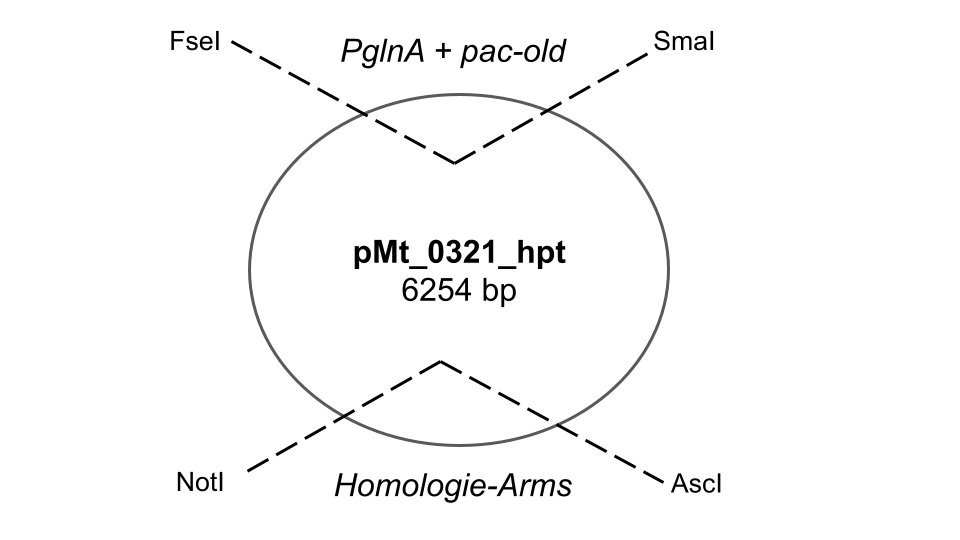
\includegraphics[width = \textwidth]{figures/Results/BC/pMt_0321_hpt}
	\end{subfigure}
	
	\vspace{0.5cm}
	
	\begin{subfigure}[b]{0.45\textwidth}
		\centering
		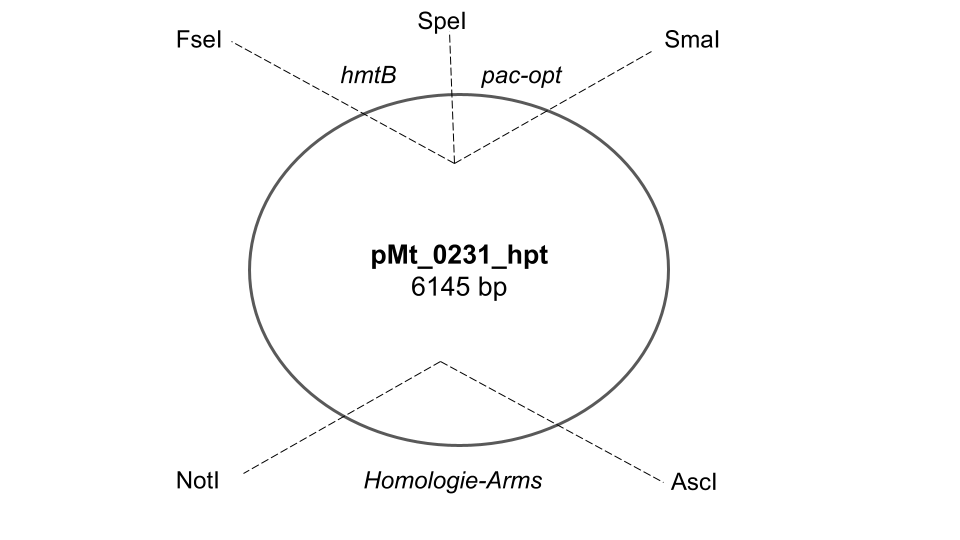
\includegraphics[width = \textwidth]{figures/Results/BC/pMt_0231_hpt_karte}
	\end{subfigure}
	\begin{subfigure}[b]{0.45\textwidth}
		\centering
		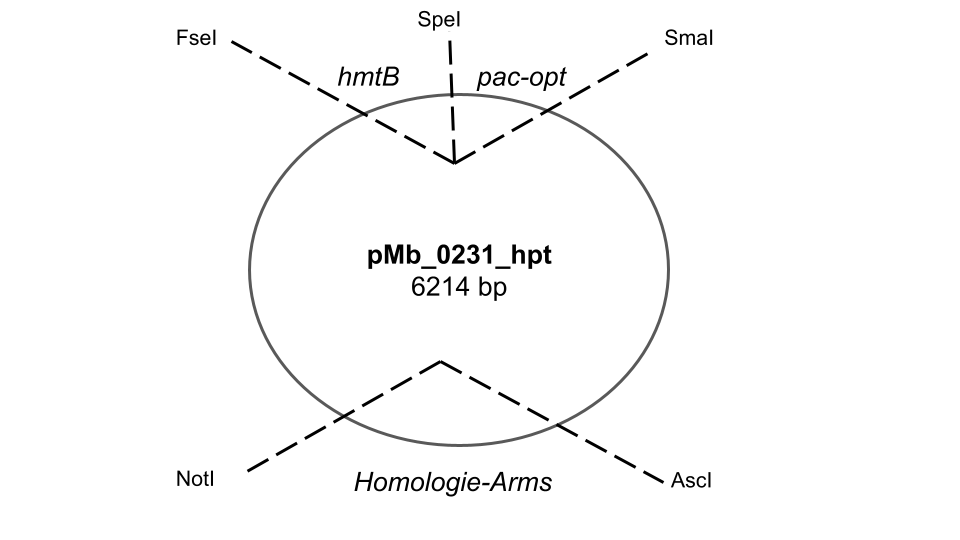
\includegraphics[width = \textwidth]{figures/Results/BC/pMb_0231_hpt}
	\end{subfigure}
	\caption[Suicide plasmid maps for transformation by \gls{conjug} for \acrshort{thau} and \acrshort{bovi}.]{Suicide plasmid maps for transformation by \gls{conjug} for \acrshort{thau} and \acrshort{bovi}. pMt\_0321\_hpt (6254~bp) is the parent plasmid used to construct the other two, pMt\_0231\_hpt (6145~bp) and pMb\_0231\_hpt (6214~bp). The maps show only the gene regions (between the dashed lines) that have been modified, as well as the \gls{rstrsite} sites (at the end of the dashed lines) used or the newly created \gls{rstrsite} sites. The new produced plasmids were verified via nanopore sequencing.}
	\label{fig:plasmid_produced}
\end{figure}

Two plasmids were constructed, as shown in \cref{fig:plasmid_produced}: pMt\_0231\_hpt for \acrshort{thau} and pMb\_0231\_hpt for \acrshort{bovi}. Compared to the plasmid originally used for the construction, a new \gls{rstrsite} (SpeI) was inserted between the \textit{pac} and its promoter (see \cref{fig:plasmid_produced}). In addition, the plasmid \textit{pac\_old}, which contained the alternative \acrshort{aa} sequence, was converted to the codon-optimized version with the original \acrshort{aa} sequence (\textit{pac\_opt}), and the promoter was changed to hmtB.\\

Both plasmids were verified by sequencing.

\subsubsection{Transformation of \textit{Methanobrevibacter}}

The \acrshort{dap}-\gls{auxo} \acrshort{ecol26} and \acrshort{ecol29} were successfully transformed with the plasmids pMt\_0231\_hpt, pMm\_0231\_hpt and pMb\_0231\_hpt. For the \gls{conjug} each plasmid combination with \acrshort{ecol26} and \acrshort{ecol29} were cultivated in 20~ml~LB~media with 0.1~mM~\acrshort{dap} and 30~µg/ml~chloramphenicol. For all \acrlong{mbrevi} species except \acrshort{bovi}* the media was inoculated with 1~ml \acrshort{ecol26} and WM6029 pre-culture and cultivated for 4.5~h. For \acrshort{bovi}, it was inoculated with 1.5~ml and the \acrshort{ecol} were cultivated for 3.75~h. The final \acrshort{OD} is shown in \cref{tab:conjugation_preparation}.

For the growth of \acrshort{ecol26} and WM6029 is quit heterogenous. So have the strains with 1~ml inoculation final \acrshort{OD} values between 1.02 and 1.59. The maximum \acrshort{OD} (1.79) was measured for WM6026 with 1.5~ml inoculation and a 45~min shorter cultivation. But the minimum was measured for this preparation as well with 0.60 for WM6029.\\

For the \gls{conjug} 28 preparations were prepared (see \cref{tab:conjugation_preparation}). They differ in combination of \acrshort{ecol} strain and \acrlong{mbrevi} species (cultures with an asterisk showed first visual growth on the day they were used for the \gls{conjug}) and in the recovery-time (time until \acrfull{puro} was added, see t\textsubscript{P} in \cref{tab:conjugation_preparation}) as well as in the time until then they were transferred in new selection media (see t\textsubscript{1\_t} and t\textsubscript{2\_t} in \cref{tab:conjugation_preparation}).\\



%%%%%%%%%%%%%%%%%%%%%%%%%%%%%%%%%%%%%%%%%%%%%%%%%%%%
%%%%%%%%%%%%%%%%%%%%%%%%%%%%%%%%%%%%%%%%%%%%%%%%%%%%
%%%%%%%%%%%%%%%%%%%%%%%%%%%%%%%%%%%%%%%%%%%%%%%%%%%%
%%%%%%%%%%%%%%%%%%%%%%%%%%%%%%%%%%%%%%%%%%%%%%%%%%%%
%%%%%%%%%%%%%%%%%%%%%%%%%%%%%%%%%%%%%%%%%%%%%%%%%%%%
%%%%%%%%%%%%%%%%%%%%%%%%%%%%%%%%%%%%%%%%%%%%%%%%%%%%

%%%%%%%%%%%%%%%%%%%%%%%%%%%%%%%%%%%%%%%%%%%%%%%%%%%%


\subsection{Geography}

The general methodology for the processing, analyses and visualization of the CRT data in R was to build a function and then apply these with the interested variables and data from the specific countries.
In the following part, the general procedure is described in the part below. For a more detailed overview, please check the R scripts.

\subsubsection{Processing CRT-Data} 
\label{sec:processing_CRT_DATA}

\textbf{Cattle enteric fermentation}

\noindent For \acrlong{deu} and \acrlong{nzl} all given data for cattle and its subcattegories "dairy cattle" and "non-dairy cattle" were imported from the "Table3.A" sheet of th CRT tables for each year, and processed so, that for each year of each country a table was created with one column with the year, one column with the cattle type and the following columns are for the measured or calculated values. Afterwards, all one year tables of one country were merged, so that one country has one table, where the values for the cattle categories from 1990 to the last published year are present. 

For the U.S. there are no direct "Dairy cattle" and "Non-dairy cattle" categories, but more detailed one. So after the import of the same value columns for each cattle category as described before, these more detailed subcategories have to be merged in the same 2 as for \acrlong{deu} and \acrlong{nzl}. For this purpose, the official definition and classifications from the U.S. \citep[Chapter 5, p.\,6]{epaInventoryUSGreenhouse2024} were used. DE, GE and Ym were merged as a weighted mean with the populations as weight. The methane emission were summed.\\

\textbf{Methane emission for each sector}

\noindent For sector-specific emissions, only the “TableS3” sheet was used for the most recent CRT (for the U.S., the year 2022; for Germany and New Zealand, the year 2024). Here, all sectors and their subcategories were imported for all years, as were the total emissions. After processing the data, only the methane emission values for the sectors in general were retained, as well as the total methane emissions for each country.

\subsubsection{Calculation of methane emissions from enteric fermentation processes in cattle}
\label{sec:methane_emis_calc_method}

The total methane emission for cattle and its subcategories dairy and non-dairy was not directly extracted from the published \acrfull{crt} for the countries, but calculated from the indicators \acrfull{Ym}, \acrfull{GE} and the population number of the animal categories. Therefore, the \ch{CH4} emissions were calculated for dairy and non-dairy cattle following the \cref{eq:emission_total}. The methane emission for cattle than is the sum of dairy and non-dairy.


\begin{equation}
CH_{4,T} = \frac{GE\cdot (\frac{Ym}{100})\cdot 365}{55.65}\cdot \frac{N_T}{10^6}
	\label{eq:emission_total}
\end{equation}

\noindent where:
\begin{itemize}
	\item $CH_{4, T}$ = yearly methane emission of a animal category [kt CH$_4$ year$^{-1}$]
	\item $GE$ = gross energy intake [MJ head$^{-1}$ day$^{-1}$]
	\item $Ym$ = methane conversion factor [\%]
	\item $55.65$ = energy content of \ch{CH4} [MJ kg$^{-1}$]
	\item $N_T$ = population-size of animal category
	\item $10^6$ = conversion-factor kg to kt
\end{itemize}


%%%%%%%%%%%%%%%%%%%%%%%%%%%%%%%%%%%%%%%%%%%%%%%%%%%%%%%%%%%%%%%%%%%%%%%%%%%%%
%%%%%%%%%%%%%%%%%%%%%%%%%%%%%%%%%%%%%%%%%%%%%%%%%%%%%%%%%%%%%%%%%%%%%

\subsubsection{Share of cattle methane emissions from enteric fermentation}

 The share of enteric fermentation was claculated for its fraction on the total amount of anthropogen produced \ch{CH4} in a country and on the methane emissions resulting from the agriculture sector. For this purpose the published data in the CRT was used for each country. 

%%%%%%%%%%%%%%%%%%%%%%%%%%%%%%%%%%%%%%%%%%%%%%%%%%%%%%%%%%%%%%%%%%%%%%%%%%%%%
%%%%%%%%%%%%%%%%%%%%%%%%%%%%%%%%%%%%%%%%%%%%%%%%%%%%%%%%%%%%%%%%%%%%%

\subsubsection{Calculation of saved methane}
\label{sec:methods-calc_saved_methane}

To calculate the potential methane savings resulting from the mitigation strategy under investigation (vaccination of cattle), various success scenarios are defined: 10, 20, 30, 40, and 50\% shifts in the rumen microbiome of cattle from methanogens toward non-methane-producing microbes.

These will have an impact on two indicators used in \citet{IPCC_2019_Chapter_EnterFE}. Ym, which represents the proportion of energy or feed consumed by cattle that is converted into methane by that microbiome, and DE, assuming that the reduced amount of feed energy converted into methane now benefits the animal during digestion, meaning that the percentage of feed digestibility for the animal increases. \\

The values of the resulting Ym (Ym\textsubscript{Red}) and DE (DE\textsubscript{Red}) are calculated as in \cref{eq:Ym_red_sze_calc} and \cref{eq:DE_red_sze_calc}.

\begin{equation}
	Ym_{Red} = Ym \cdot \left(1 - \frac{Red}{100} \right)
	\label{eq:Ym_red_sze_calc}
\end{equation}

\noindent where:
\begin{itemize}
	\item $Ym_{Red}$ = adjusted Ym for the investigated reduction scenario [\%]
	\item $Ym$ = original methane conversion factor from CRT [\%]
	\item $Red$ = investigated reduction scenario [\%]
\end{itemize}

\begin{equation}
	DE_{Red} = DE + \left( Ym \cdot \frac{Red}{100}\right)
	\label{eq:DE_red_sze_calc}
\end{equation}

\noindent where:
\begin{itemize}
	\item $DE_{Red}$ = adjusted DE for the investigated reduction scenario [\%]
	\item $DE$ = Digestibility of feed as a fraction of gross energy intake [\%] 
	\item $Red$ = investigated reduction scenario [\%]
\end{itemize}

\noindent The \cref{eq:emission_total} presents the relation of Ym and methane emission of cattle already. DE, on the other hand, is named in three different equations in the calculation of \citet{IPCC_2019_Chapter_EnterFE}, shown in the \cref{eq:GE_berechnung} through (\ref{eq:REG_calculation}) with little adjustments. It has his impact on produced methane through his role in calculate the GE of the animal, which has a linear relation towards methane emission (see \cref{eq:emission_total}).

\begin{equation}
GE = \frac{\left( \frac{NE_x}{REM}\right) +\left( \frac{NE_y}{REG}\right)}{\left( \frac{DE}{100}\right) }
\label{eq:GE_berechnung}
\end{equation}

\noindent where:
\begin{itemize}
	\item $GE$ = gross energy intake [MJ head$^{-1}$ day$^{-1}$]
	\item $NE_x$ = sum of the net energy required for maintenance ($NE_m$), for the activity ($NE_a$), for lactation ($NE_l$), for the work ($NE_work$) and for the pregnancy ($NE_p$) of the animal [MJ head$^{-1}$ day$^{-1}$]
	\item $REM$ = ratio of net energy available in a diet for maintenance (\Cref{eq:REM_calculation})
	\item $NE_y$ = sum of the net energy required for growth and for wool production [MJ head$^{-1}$ day$^{-1}$]
	\item $REG$ = ratio of net energy available for growth in a diet (\Cref{eq:REG_calculation})
	\item $DE$ = Digestibility of feed as a fraction of gross energy intake [\%] 
\end{itemize}

\begin{equation}
REM = \left[1.123 - (4.092 \cdot 10^{-3} \cdot DE) + (1.126\cdot 10^{-5} \cdot DE^{2}) - \left( \frac{25.4}{DE}\right) \right]
\label{eq:REM_calculation}
\end{equation}

\noindent where:
\begin{itemize}
	\item $REM$ = ratio of net energy available in a diet for maintenance
	\item $DE$ = Digestibility of feed as a fraction of gross energy intake [\%] 
\end{itemize}

\begin{equation}
	REM = \left[1.164 - (5.16 \cdot 10^{-3} \cdot DE) + (1.308\cdot 10^{-5} \cdot DE^{2}) - \left( \frac{37.4}{DE}\right) \right]
	\label{eq:REG_calculation}
\end{equation}

\noindent where:
\begin{itemize}
	\item $REG$ = ratio of net energy available for growth in a diet
	\item $DE$ = Digestibility of feed as a fraction of gross energy intake [\%] 
\end{itemize}

\noindent To calculate the new methane emission for cattle corresponding to the reduction scenario now, GE has to be recalculated with the adjusted DE. Afterwards \cref{eq:emission_total} can be used again to calculate the adjusted \ch{CH4} emission with the adjusted GE (GE\textsubscript{Red}) and Ym\textsubscript{Red}. 

For calculation the GE\textsubscript{Red} DE\textsubscript{Red} can not just simply be put in the \cref{eq:GE_berechnung}, because of the values for NE\textsubscript{x} and NE\textsubscript{y}. Although the values for the individual net energy intake categories (see \cref{eq:GE_berechnung}) should not change, these are not given in the published CRTs of the countries. 
To solve this problem, two things are assumed:
\begin{enumerate}
	\item The net energy required for wool production an irrelevant categorie is for the investigation of cattle.
	\item Most of the animal in the population of dairy and non-dairy cattle are fully grown or close to it. Here, too, the IPCC only classifies calves "dairy" or "non-dairy" once they started eating solid food. Because of that the net energy needed for growth will overlooked and set to 0. 
\end{enumerate}

\noindent So, the \cref{eq:GE_berechnung} can be slimmed down and rearranged to calculate a fix value for NE\textsubscript{x} for the corresponding year, because the part with NE\textsubscript{y} turns zero (see \cref{eq:NE_x_calc}).

\begin{equation}
	NE_x = GE \cdot REM \cdot \left( \frac{DE}{100}\right)
	\label{eq:NE_x_calc} 
\end{equation}

\begin{equation}
	GE = \frac{\left( \frac{NE_x}{REM}\right) }{\left( \frac{DE}{100}\right)}
	\label{eq:GE_adjusted_calc}
\end{equation}

\noindent where:
\begin{itemize}
	\item $NE_x$ = sum of the net energy required for maintenance ($NE_m$), for the activity ($NE_a$), for lactation ($NE_l$), for the work ($NE_work$) and for the pregnancy ($NE_p$) of the animal [MJ head$^{-1}$ day$^{-1}$]
	\item $GE$ = gross energy intake [MJ head$^{-1}$ day$^{-1}$] (\cref{eq:GE_berechnung})
	\item $REM$ = ratio of net energy available in a diet for maintenance (\Cref{eq:REM_calculation})
	\item $DE$ = Digestibility of feed as a fraction of gross energy intake [\%] 
\end{itemize}

\noindent Now, GE\textsubscript{Red} can be calculated for a given year using the fixed values for NE\textsubscript{x} and DE\textsubscript{Red}, all due to the assumption that NE\textsubscript{y} is 0 (see \cref{eq:GE_adjusted_calc}). The calculated gross energy intake is then substituted into \cref{eq:emission_total} along with the corresponding Ym\textsubscript{Red} value. This yields the methane emissions (\ch{CH4}\textsubscript{,R}) for a cattle category under a reduction scenario for a specific year. \\
The saved methane emissions (\ch{CH4}\textsubscript{,S}) for a specific reduction scenario are calculated by subtracting the original value for methane emissions from the value adjusted for the scenario (see \cref{eq:saved_CH4})

\begin{equation}
	CH_{4,S} = CH_{4,T} - CH_{4,R}
	\label{eq:saved_CH4}
\end{equation}

\noindent where:
\begin{itemize}
	\item $CH_{4, S}$ = saved \ch{CH4} through reduction scenario [kt CH$_4$ year$^{-1}$]
	\item $CH_{4, T}$ = yearly methane emission of a animal category [kt CH$_4$ year$^{-1}$]
	\item $CH_{4, R}$ = yearly methane emission of a animal category for a corresponding reduction scenario [kt CH$_4$ year$^{-1}$]
\end{itemize}

\subsubsection{Prediction of \ch{CH4} emission until 2030}
\label{sec:Prediction_CH4_2030}

Two steps are required to calculate total methane emissions, as well as methane emissions for three reduction scenarios (10, 30, and 50) through the year 2030.\\ 

First, total methane emissions without emissions from \acrshort{enterfe} processes in cattle are calculated and then extrapolated.\\

Second, to calculate the methane emission from \acrfull{enterfe} in cattle, the values for DE, Ym, Population size and NE\textsubscript{x} were predicted for each subcategorie ("dairy" and "non-dairy cattle") until 2030. For that, NE\textsubscript{x} had to be first calculated (see \cref{eq:NE_x_calc}). From the predicted values for these indicators the cattle \acrshort{enterfe} \ch{CH4} emission could be calculated (via \cref{eq:GE_adjusted_calc} and (\ref{eq:emission_total})).

Also the the methane emission values for three different reduction scenarios (10, 30 and 50) were calculated with these values using the \cref{eq:Ym_red_sze_calc}, (\ref{eq:DE_red_sze_calc}), (\ref{eq:GE_adjusted_calc}) and (\ref{eq:emission_total}).

Afterwards, the emissions of the subcategories were summed to the \ch{CH4} emission for cattle resulting from enteric fermentation processes.\\

Third, the predicted emission values for total without cattle enteric fermentation were added with the calculated emission values for cattle enteric fermentation to achieve the total methane emission of a country.\\

The forecast was made using a linear regression, with the value to be predicted depending on the respective year. However, the regression was not based on the entire time period, but rather on three different time intervals (the last 5, 10, and 15 years). For each linear model, both the \acrfull{ci} with a confidence level of 95\% and the total emissions were calculated. In addition, the R\textsuperscript{2} value was determined for each model.\\

The extrapolation extends from 2025 to 2030 for \acrlong{nzl} and \acrlong{deu}, and from 2023 to 2030 for \acrshort{usa}.
